%!TEX root = main.tex

\section{Analysis of Web Search Flows}
\label{sec:web_search}

% In this section, 

\subsection{Analysis Framework}

We divide the analysis of web search flow into 3 different pieces corresponding to the three subsequent stages: \emph{3-way handshake}, \emph{slow start}, \emph{congestion avoidance}, in which web server has different transmission strategies.

In TCP 3-way handshake, server establishes connection with client, in preparation for data transmission. Ideally, this stage completes in 1 RTT. However, in the dataset we could see that a non-negligible fraction of flows experience SYN retransmission in 3-way handshake. In slow start stage, server does not encounter packet loss or reordering event. Thus it enlarges the congestion window by 1 segment size for each received acknowledgment, and transmits data constrained by the window size. Server leaves slow start and enters congestion avoidance stage when it encounters congestion event, like packet loss or reordering. In congestion avoidance stage, server reduces the congestion window when detecting packet loss through fast retransmit\cite{jacobson1988congestion} and compels the congestion window to grow from 1 segment size when detecting packet loss through RTO. If there is no congestion event, the flow will complete in slow start stage. It is worth noting that, different from the TCP congestion avoidance state in TCP/IP stack, the \emph{congestion avoidance} stage here starts when server detects congestion event and ends till the flow finishes. 

The three stages could be exemplified in Figure~\ref{fig:web_three_stages}, which shows the time-line and sequence number of a real flow in web search. In the figure, server takes 1.8s to establish connection, 3.1s to transmit 35 data packets in slow start stage, and 15.3s to transmit the left 48 data packets in congestion avoidance stage.

\begin{figure}[th]
\centering
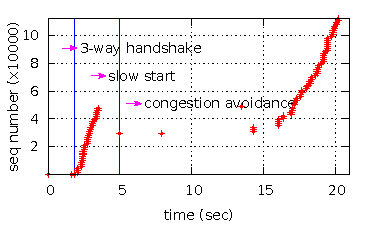
\includegraphics[width=\linewidth]{web_three_stages}
\caption{The three stages in web search flows.}
\label{fig:web_three_stages}
\end{figure}

\subsection{Causal Analysis of Transmission Speed}

\begin{figure}[th]
\centering
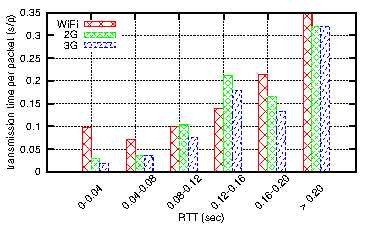
\includegraphics[width=\linewidth]{web_rtt}
\caption{The average transmission speed under different RTT's.}
\label{fig:web_rtt}
\end{figure}

First, we investigate the impact of RTT on the performance metric of web search flows: transmission speed. We also use 0.4s interval to group the flows by their RTT's. The result is shown in Figure~\ref{fig:web_rtt}. From the figure, as the RTT value becomes larger, the overall transmission speed grows correspondingly. For smaller RTT value (less than 0.08s), the normalized finish time of flows in WiFi network is 1-4 times larger than that of flows in cellular network. When the RTT value is larger than 0.08s, flows in all networks have similar normalized finish time. Note that most of flows (95\%) in cellular network have RTT smaller than 0.08s, which verifies that the normalized finish time of flows in cellular is much better than that of flows in WiFi network in Figure~\ref{fig:web_finish_time}.

\begin{table}[th]
\centering
\renewcommand{\arraystretch}{1.2}
\caption{Normalized finish time under different RTT values in cellular network using QED.}
\label{tab:web_cellular_rtt_qed}
\begin{tabular}{l|c|c}
\toprule
RTT bin (s) & 2G & 3G \\
\midrule
$[$ 0.01, 0.02 ) & 11.1 & 6.6 \\
\hline
$[$ 0.02, 0.03 ) & 28.0 & 32.3 \\
\hline
$[$ 0.03, 0.04 ) & 25.1 & 22.4 \\
\hline
$[$ 0.04, 0.05 ) & 67.0 & 59.2 \\
\hline
$[$ 0.05, 0.06 ) & 60.5 & 59.0 \\
\hline
$[$ 0.06, 0.07 ) & 38.6 & 38.8 \\
\hline
$[$ 0.07, 0.08 ) & 69.7 & 39.0 \\
\hline
$[$ 0.08, $\infty$ ) & 581.8 & 317.6 \\
\bottomrule
\end{tabular}
\end{table}

Due to the different distribution of RTT's in cellular network and WiFi network, we investigate the impact of RTT separately. In cellular network data, we use 0.01s interval to group the flows into 9 bins, and take the flows in bin $[$ 0, 0.01 ) as the baseline. For each flow in the baseline, we randomly choose such a flow which has the same access type, the same number of lost packets, and the same condition whether encountering RTO, in each of other bins, and compute the ratio of their normalized finish time to that of the baseline flow. The results are shown in Table~\ref{tab:web_cellular_rtt_qed}. From the table, the normalized finish time of flows with RTT larger than 0.01s is much larger than that of flow with RTT smaller than 0.01s. However, we could not find the evidence in the table that normalized finish time is proportional to RTT value in web search. We also use 0.01s interval to bin the flows in WiFi network into 21 groups. The results are not shown due to space limit. In WiFi network, when the RTT is between 0.04s and 0.16s, the normalized finish time is not proportional to RTT, either. 

\begin{figure}[th]
\centering
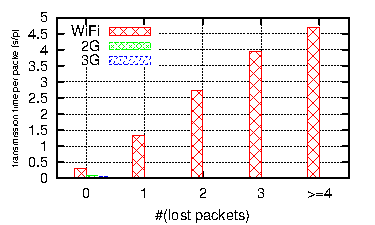
\includegraphics[width=\linewidth]{web_loss_finish_time}
\caption{Normalized finish time under different number of lost packets.}
\label{fig:web_loss_finish_time}
\end{figure}

Next, we investigate the impact of packet loss on the normalized finish time. Note that the packet loss rate in 2G/3G network is less than 0.005\%, thus the impact in cellular network could be omitted. In contrast, about 5\% of flows in WiFi network encounter packet loss. Figure~\ref{fig:web_loss_finish_time} plots the normalized finish time under different number of lost packets. In the figure, when there is no packet loss, the performance of each access type could be ranked as: 3G $>$ 2G $>>$ WiFi. In WiFi network, when the number of lost packets is larger than 3, the normalized finish time is 15 times larger than that with no packet loss.

\begin{figure}[th]
\centering
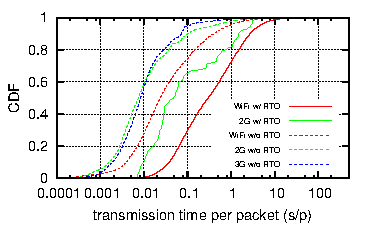
\includegraphics[width=\linewidth]{web_timeout}
\caption{Normalized finish time of flows with and without timeout retransmission.}
\label{fig:web_timeout}
\end{figure}

Even though flows in 2G network seldom encounters packet loss, 0.7\% of them suffer from timeout retransmission due to packet delay or lost acknowledgment. Figure~\ref{fig:web_timeout} shows the normalized finish time of flows with and without timeout retransmission. In the figure, under the same access type (WiFi and 2G network), the normalized finish time of flows with timeout retransmission is one order of magnitude larger than those without timeout retransmission. Considering flows with timeout retransmission, flows in 2G network have shorter normalized finish time than those in WiFi network. The reasons are as follows. First, flows in 2G network have smaller RTT, and thus smaller RTO according to \cite{rfc62982011computing}. Second, many timeout retransmissions in 2G network are spurious due to packet delay or lost acknowledgment. When receiving Duplicate SACK if the first packet is not dropped, server recovers the original congestion window using F-RTO~\cite{sarolahti2005forward}, instead of increasing the window from 1 segment size.


